%!TEX root = foglio.tex

\tikzset{every picture/.style={line width=0.75pt}} %set default line width to 0.75pt        

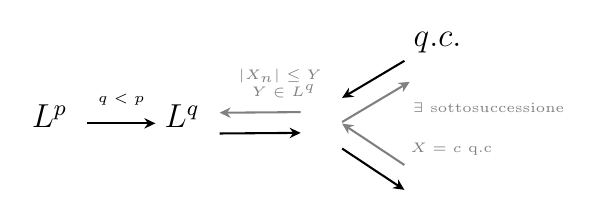
\begin{tikzpicture}[x=0.75pt,y=0.75pt,yscale=-1,xscale=1]
%uncomment if require: \path (0,119); %set diagram left start at 0, and has height of 119

% Text Node
\draw (14,50.4) node [anchor=north west][inner sep=0.75pt]  [font=\large]  {$L^{p}$};
% Text Node
\draw (78,50.4) node [anchor=north west][inner sep=0.75pt]  [font=\large]  {$L^{q}$};
% Text Node
\draw (148,50.9) node [anchor=north west][inner sep=0.75pt]  [font=\large]  {$\PP$};
% Text Node
\draw (198,85.4) node [anchor=north west][inner sep=0.75pt]  [font=\large]  {$\Lc$};
% Text Node
\draw (198,15.4) node [anchor=north west][inner sep=0.75pt]  [font=\large]  {$\text{q.c.}$};
% Text Node
\draw (46,45.4) node [anchor=north west][inner sep=0.75pt]  [font=\tiny]  {$q< p$};
% Text Node
\draw (107,32.9) node [anchor=north west][inner sep=0.75pt]  [font=\tiny,color={rgb, 255:red, 128; green, 128; blue, 128 }  ,opacity=1 ]  {$ \begin{array}{l}
| X_{n}| \leq Y\\
\ \ Y\in L^{q}
\end{array}$};
% Text Node
\draw (197.5,49.5) node [anchor=north west][inner sep=0.75pt]  [font=\tiny,color={rgb, 255:red, 128; green, 128; blue, 128 }  ,opacity=1 ] [align=left] {$\exists $ sottosuccessione};
% Text Node
\draw (196.5,69) node [anchor=north west][inner sep=0.75pt]  [font=\tiny,color={rgb, 255:red, 128; green, 128; blue, 128 }  ,opacity=1 ] [align=left] {$X=c$ q.c};
% Connection
\draw    (42,61) -- (72,61) ;
\draw [shift={(75,61)}, rotate = 180] [fill={rgb, 255:red, 0; green, 0; blue, 0 }  ][line width=0.08]  [draw opacity=0] (5.36,-2.57) -- (0,0) -- (5.36,2.57) -- (3.56,0) -- cycle    ;
% Connection
\draw [color={rgb, 255:red, 128; green, 128; blue, 128 }  ,draw opacity=1 ]   (109,55.86) -- (145,55.58) ;
\draw [shift={(106,55.88)}, rotate = 359.56] [fill={rgb, 255:red, 128; green, 128; blue, 128 }  ,fill opacity=1 ][line width=0.08]  [draw opacity=0] (5.36,-2.57) -- (0,0) -- (5.36,2.57) -- (3.56,0) -- cycle    ;
% Connection
\draw [color={rgb, 255:red, 0; green, 0; blue, 0 }  ,draw opacity=1 ]   (142,65.6) -- (106,65.88) ;
\draw [shift={(145,65.58)}, rotate = 179.56] [fill={rgb, 255:red, 0; green, 0; blue, 0 }  ,fill opacity=1 ][line width=0.08]  [draw opacity=0] (5.36,-2.57) -- (0,0) -- (5.36,2.57) -- (3.56,0) -- cycle    ;
% Connection
\draw    (167.58,47.2) -- (195,30.89) ;
\draw [shift={(165,48.73)}, rotate = 329.25] [fill={rgb, 255:red, 0; green, 0; blue, 0 }  ][line width=0.08]  [draw opacity=0] (5.36,-2.57) -- (0,0) -- (5.36,2.57) -- (3.56,0) -- cycle    ;
% Connection
\draw [color={rgb, 255:red, 128; green, 128; blue, 128 }  ,draw opacity=1 ]   (194.98,42.53) -- (165,60.37) ;
\draw [shift={(197.56,41)}, rotate = 149.25] [fill={rgb, 255:red, 128; green, 128; blue, 128 }  ,fill opacity=1 ][line width=0.08]  [draw opacity=0] (5.36,-2.57) -- (0,0) -- (5.36,2.57) -- (3.56,0) -- cycle    ;
% Connection
\draw [color={rgb, 255:red, 128; green, 128; blue, 128 }  ,draw opacity=1 ]   (167.5,62.79) -- (195,81.04) ;
\draw [shift={(165,61.13)}, rotate = 33.56] [fill={rgb, 255:red, 128; green, 128; blue, 128 }  ,fill opacity=1 ][line width=0.08]  [draw opacity=0] (5.36,-2.57) -- (0,0) -- (5.36,2.57) -- (3.56,0) -- cycle    ;
% Connection
\draw    (192.5,91.38) -- (165,73.13) ;
\draw [shift={(195,93.04)}, rotate = 213.56] [fill={rgb, 255:red, 0; green, 0; blue, 0 }  ][line width=0.08]  [draw opacity=0] (5.36,-2.57) -- (0,0) -- (5.36,2.57) -- (3.56,0) -- cycle    ;

\end{tikzpicture}